\lecture{IAS Computer}{2023-01-30}{16:00}{Farzad}{RB LT1}

\section{IAS Computer}
The IAS Computer uses the stored program concept. This is where the instructions and data required to execute the program are stored in the computer's main memory then during runtime moved to the CPU where each instruction is executed one by one.

Further details on the IAS computer's structure can be found in the previous lecture. 

There are three key concepts of the IAS Computer
\begin{itemize}
    \item Single read-write memory (data and instructions both stored here)
    \item Memory is addressable
    \item Execution occurs in a sequential fashion (unless explicitly modified)
\end{itemize}

\section{Registers}
Registers are very small amounts of very fast and expensive memory which is found within the CPU. There are a number of registers and each have a specific purpose. 

\begin{description}
    \item[Memory Buffer Register (MBR)] contains a word to be stored in memory or sent to the I/O unit; or used to receive a word from memory or from the I/O unit.
    \item[Memory Address Register (MAR)] specifies the address in memory of the word to be written from or read into the MBR.
    \item[Instruction Register (IR)] contains the 8-bit opcode from the instruction currently being executed.
    \item[Program Counter (PC)] contains the the address of the next instruction pair to be fetched from memory
    \item[Accumulator (AC) and Multiplier Quotient (MQ)] are used to hold operands temporarily and results of ALU operations. MQ gets used if the results from the ALU is too big to fit in the AC.
\end{description} 

\begin{figure}[H]
    \centering
    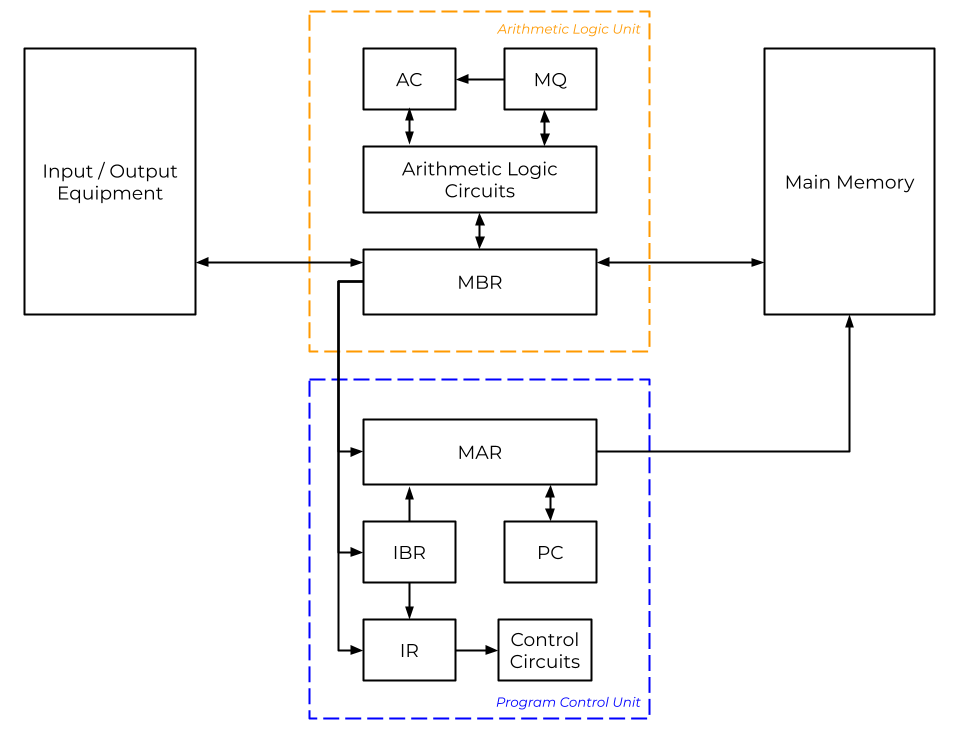
\includegraphics[width=0.7\textwidth]{assets/ias-registers.png}
    \caption{IAS Registers}
\end{figure}

\section{Instructions}
The IAS Computer had a very limited set of instructions.
\begin{table}[H]
    \centering
    \begin{tabularx}{\textwidth}{XXX}
        \textbf{Opcode} & \textbf{Symbolic Representation} & \textbf{Description}\\
    \end{tabularx}
\end{table}

\subsection{Data Transfer}
\begin{table}[H]
    \centering
    \begin{tabularx}{\textwidth}{XXX}
        \hline
        \texttt{00001010} & \texttt{LOAD MQ} & Transfer the contents of register \texttt{MQ} to the accumulator \texttt{AC}\\
        \hline
        \texttt{00001001} & \texttt{LOAD MQ,M(X)} & Transfer the contents of memory location \texttt{X} to \texttt{MQ}\\
        \hline
        \texttt{00100001} & \texttt{STOR M(X)} & Transfer contents of accumulator to memory location \texttt{X}\\
        \hline
        \texttt{00000001} & \texttt{LOAD M(X)} & Transfer \texttt{M(X)} to the accumulator\\
        \hline
        \texttt{00000010} & \texttt{LOAD-M(X)} & Transfer \texttt{-M(X)} to the accumulator\\
        \hline
        \texttt{00000011} & \texttt{LOAD |M(X)|} & Transfer absolute value of \texttt{M(X)} to the accumulator\\
        \hline
        \texttt{00000100} & \texttt{LOAD -|M(X)|} & Transfer \texttt{-|M(X)|} to the accumulator\\
        \hline
    \end{tabularx}
\end{table}

\subsection{Unconditional Branch}
\begin{table}[H]
    \centering
    \begin{tabularx}{\textwidth}{XXX}
        \hline
        \texttt{00001101} & \texttt{JUMP M(X,0:19)} & Take next instruction from left half of \texttt{M(X)}\\
        \hline
        \texttt{00001110} & \texttt{JUMP M(X,20:39)} & Take next instruction from right half of \texttt{M(X)}\\
        \hline
    \end{tabularx}
\end{table}

\subsubsection{Conditional Branch}
\begin{table}[H]
    \centering
    \begin{tabularx}{\textwidth}{XXX}
        \hline
        \texttt{00001111} & \texttt{JUMP+M(X,0:19)} & If number in the accumulator is non-negative, take next instruction from left half of \texttt{M(X)}\\
        \hline
        \texttt{00010000} & \texttt{JUMP+M(X,20:39)} & If number in the accumulator is non-negative, take the next instruction from the right half of \texttt{M(X)}\\
        \hline
    \end{tabularx}
\end{table}

\subsection{Arithmetic}
\begin{table}[H]
    \begin{tabularx}{\textwidth}{XXX}
        \hline
        \texttt{00000101} & \texttt{ADD M(X)} & Add \texttt{M(X)} to AC; pur result in AC\\
        \hline
        \texttt{00000111} & \texttt{ADD |M(X)|} & Add \texttt{|M(X)|} to AC; put result in AC\\
        \hline
        \texttt{00000110} & \texttt{SUB M(X)} & Subtract \texttt{M(X)} from AC; put result in AC\\
        \hline
        \texttt{00001000} & \texttt{SUB |M(X)|} & Subtract \texttt{SUB |M(X)|} from AC; put the remainder in AC\\
        \hline
        \texttt{00001011} & \texttt{MUL M(X)} & Multiply \texttt{M(X)} by MQ; put MSBs in AC, put LSBs in MQ\\
        \hline
        \texttt{00001100} & \texttt{DIV M(X)} & Divide AC by \texttt{M(X)}; put quotient in MQ and remainder in AC\\
        \hline
        \texttt{00010100} & \texttt{LSH} & Multiple AC by 2 (left shift by 1 position)\\
        \hline
        \texttt{00010101} & \texttt{RSH} & Divide AC by 2 (right shift by 1 position)\\
        \hline
    \end{tabularx}
\end{table}

\subsection{Address Modify}
\begin{table}[H]
    \begin{tabularx}{\textwidth}{XXX}
        \hline
        \texttt{00010010} & \texttt{STOR M(X,8:19)} & Replace left address field at \texttt{M(X)} by 12 rightmost bits of AC\\
        \hline
        \texttt{00010011} & \texttt{STOR M(X,28:39)} & Replace right address field at \texttt{M(X)} by 12 rightmost bits of AC\\
        \hline        
    \end{tabularx}
\end{table}


\section{Programs}
There are two different methods of programming computers, that we need to know about at this stage.
\subsection{Hardwired Programs}
This is like what we did in \texttt{logic.ly}. This is where the individual logic gates inputs are hand-manipulated and the connections are put together by hand to generate outputs.

\subsection{Software Programming}
This works by the code being written in a language which then gets passed through an interpreter. The interpreter will translate the high level language into a low level language which the components of the computer are able to understand and use. 